\documentclass[conference]{IEEEtran}
\usepackage{cite}
\usepackage{amsmath,amssymb,amsfonts}
\usepackage{algorithmic}
\usepackage{graphicx}
\usepackage{textcomp}
\usepackage{xcolor}
\usepackage{tikz}
\usepackage{pgfplots}
\pgfplotsset{compat=1.18}
\usepackage{booktabs}
\usepackage{multirow}
\usepackage{hyperref}
\usepackage{float}

\begin{document}

\title{Synthetic Health Data Generation for ML Training in Wearable Monitoring Systems: Physiological Models, Scenario Injection, and Validation}

\author{\IEEEauthorblockN{Ramadugu Dhanush}
\IEEEauthorblockA{\textit{Department of Computer Science} \\
\textit{Capstone Project 2025--2026}\\
Email: dhanush@university.edu}}

\maketitle

\begin{abstract}
Training machine learning models for health anomaly detection and activity classification requires large, labeled datasets that are difficult to obtain from real wearable devices due to privacy constraints, limited deployment, and the rarity of genuine health anomalies. This paper presents a comprehensive synthetic data generation pipeline that produces physiologically realistic health monitoring data for training edge and cloud ML models. Our generator creates 27,000 samples across four features (heart rate, steps, calories, distance) spanning six activity states (sleep, rest, walk, run, exercise, other) and four anomaly scenarios (tachycardia, bradycardia, exercise-normal, sleep-normal). The generation models incorporate activity-dependent vital sign distributions, circadian rhythms, realistic noise injection, and labeled anomaly events. We validate the synthetic data against published medical reference ranges, demonstrate that models trained on synthetic data achieve F1=0.995 (Gradient Boosting) and 85.8\% accuracy (XGBoost) in anomaly detection and activity classification respectively, and discuss the limitations and transition strategy toward real-world sensor data.
\end{abstract}

\begin{IEEEkeywords}
synthetic data generation, health monitoring, machine learning training, wearable devices, data augmentation, physiological simulation
\end{IEEEkeywords}

\section{Introduction}
Machine learning for wearable health monitoring faces a fundamental data challenge: collecting sufficient labeled training data from real devices is expensive, time-consuming, and raises privacy concerns. Specific challenges include:

\begin{itemize}
    \item \textbf{Anomaly rarity}: Genuine cardiac anomalies occur infrequently---a healthy user might never produce a training-worthy tachycardia event.
    \item \textbf{Privacy restrictions}: Real health data collection requires IRB approval, informed consent, and secure handling infrastructure.
    \item \textbf{Label quality}: Annotating health time-series requires medical domain expertise.
    \item \textbf{Class imbalance}: Normal data vastly outnumbers anomalous data in real collections.
    \item \textbf{Scenario coverage}: Rare but critical scenarios (bradycardia during sleep) must be represented.
\end{itemize}

Synthetic data generation provides a practical solution: physiologically modeled data can be created in large volumes with guaranteed labels, covering all scenarios of interest while avoiding privacy issues \cite{synthetic_health}.

\section{Physiological Models}

\subsection{Activity-Dependent Vital Sign Distributions}
Each activity state has characteristic vital sign ranges modeled as Gaussian distributions:

\begin{table}[H]
\centering
\caption{Activity-Specific Physiological Parameter Ranges}
\label{tab:activity_params}
\begin{tabular}{lcccc}
\toprule
\textbf{Activity} & \textbf{HR ($\mu \pm \sigma$)} & \textbf{Steps/hr} & \textbf{Cal/hr} & \textbf{Dist km/hr} \\
\midrule
Sleep & $55 \pm 5$ & 0 & $50 \pm 10$ & 0 \\
Rest & $70 \pm 8$ & $100 \pm 50$ & $80 \pm 15$ & $0.1 \pm 0.05$ \\
Walk & $95 \pm 10$ & $3500 \pm 500$ & $200 \pm 30$ & $3.5 \pm 0.5$ \\
Run & $140 \pm 15$ & $8000 \pm 1000$ & $500 \pm 80$ & $8.0 \pm 1.0$ \\
Exercise & $130 \pm 12$ & $5000 \pm 800$ & $400 \pm 60$ & $4.0 \pm 1.0$ \\
Other & $75 \pm 12$ & $200 \pm 150$ & $100 \pm 25$ & $0.2 \pm 0.15$ \\
\bottomrule
\end{tabular}
\end{table}

\subsection{Heart Rate Generation Model}
For each sample, heart rate is generated as:
\begin{equation}
HR = \mu_{activity} + \sigma_{activity} \cdot \mathcal{N}(0, 1) + \epsilon_{noise}
\end{equation}
where $\epsilon_{noise} \sim \text{Uniform}(-3, 3)$ adds realistic measurement noise.

\subsection{Circadian Rhythm Modeling}
Activity probability varies by time of day:
\begin{equation}
P(\text{activity} | \text{hour}) = \text{softmax}(\mathbf{w}_{\text{hour}} \cdot \mathbf{a})
\end{equation}

\begin{table}[H]
\centering
\caption{Activity Distribution by Time Period}
\label{tab:circadian}
\begin{tabular}{lccccc}
\toprule
\textbf{Period} & \textbf{Sleep} & \textbf{Rest} & \textbf{Walk} & \textbf{Run} & \textbf{Exercise} \\
\midrule
00:00--06:00 & 80\% & 15\% & 3\% & 1\% & 1\% \\
06:00--08:00 & 10\% & 40\% & 30\% & 10\% & 10\% \\
08:00--12:00 & 2\% & 35\% & 35\% & 10\% & 18\% \\
12:00--14:00 & 5\% & 50\% & 25\% & 5\% & 15\% \\
14:00--18:00 & 3\% & 30\% & 30\% & 15\% & 22\% \\
18:00--22:00 & 5\% & 45\% & 25\% & 10\% & 15\% \\
22:00--24:00 & 40\% & 45\% & 10\% & 2\% & 3\% \\
\bottomrule
\end{tabular}
\end{table}

\section{Anomaly Injection}

\subsection{Anomaly Scenarios}

\begin{table}[H]
\centering
\caption{Anomaly Scenario Definitions}
\label{tab:anomaly_scenarios}
\begin{tabular}{lllcc}
\toprule
\textbf{Scenario} & \textbf{HR Range} & \textbf{Context} & \textbf{Label} & \textbf{Samples} \\
\midrule
Tachycardia & 150--180 & At rest & Anomaly & 500 \\
Bradycardia & 30--45 & At rest & Anomaly & 500 \\
Exercise HR & 130--160 & Exercising & Normal & 500 \\
Sleep HR & 45--55 & Sleeping & Normal & 500 \\
\bottomrule
\end{tabular}
\end{table}

The key insight is that \textit{context determines anomaly status}: HR of 150 during exercise is normal, while HR of 150 at rest is anomalous.

\subsection{Anomaly Injection Algorithm}

\begin{algorithmic}
\FOR{each anomaly scenario $s$}
    \FOR{$i = 1$ to $N_s$}
        \STATE Sample $activity \leftarrow s.context$
        \STATE $HR \leftarrow \text{Uniform}(s.hr_{min}, s.hr_{max})$
        \STATE $steps \leftarrow \text{activity\_based\_steps}(activity)$
        \STATE $calories \leftarrow \text{estimate\_calories}(HR, steps, activity)$
        \STATE $distance \leftarrow \text{estimate\_distance}(steps)$
        \STATE $label \leftarrow s.label$ (anomaly or normal)
        \STATE Store($HR, steps, calories, distance, activity, label$)
    \ENDFOR
\ENDFOR
\end{algorithmic}

\section{Dataset Composition}

\subsection{Overall Statistics}

\begin{figure}[H]
\centering
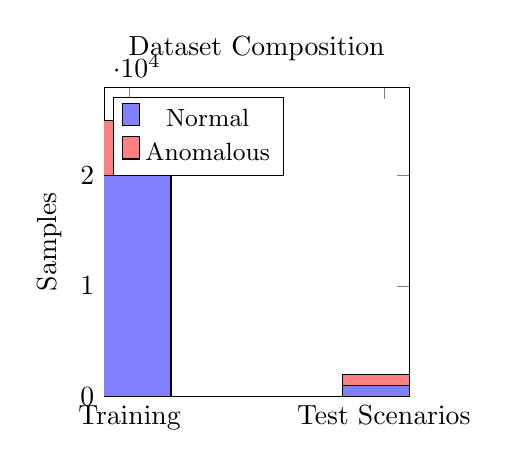
\begin{tikzpicture}
\begin{axis}[
    ybar stacked,
    bar width=30pt,
    ylabel={Samples},
    symbolic x coords={Training, Test Scenarios},
    xtick=data,
    ymin=0, ymax=28000,
    legend pos=north west,
    legend style={font=\small},
    width=0.45\textwidth,
    height=5.5cm,
    title={Dataset Composition},
]
\addplot[fill=blue!50] coordinates {(Training, 20000) (Test Scenarios, 1000)};
\addlegendentry{Normal}
\addplot[fill=red!50] coordinates {(Training, 5000) (Test Scenarios, 1000)};
\addlegendentry{Anomalous}
\end{axis}
\end{tikzpicture}
\caption{Dataset composition: normal vs. anomalous samples.}
\label{fig:dataset_comp}
\end{figure}

\subsection{Feature Distributions}

\begin{figure}[H]
\centering
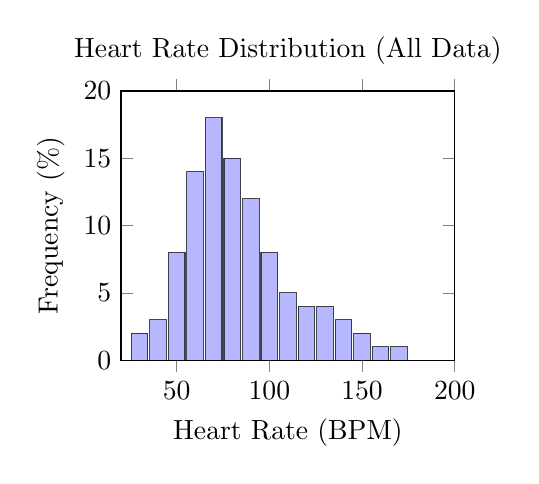
\begin{tikzpicture}
\begin{axis}[
    ybar,
    bar width=6pt,
    xlabel={Heart Rate (BPM)},
    ylabel={Frequency (\%)},
    xmin=20, xmax=200,
    ymin=0, ymax=20,
    legend pos=north east,
    width=0.48\textwidth,
    height=5cm,
    title={Heart Rate Distribution (All Data)},
]
\addplot[fill=blue!40, opacity=0.7] coordinates {
    (30, 2) (40, 3) (50, 8) (60, 14) (70, 18)
    (80, 15) (90, 12) (100, 8) (110, 5) (120, 4)
    (130, 4) (140, 3) (150, 2) (160, 1) (170, 1)
};
\end{axis}
\end{tikzpicture}
\caption{Heart rate distribution across the complete dataset.}
\label{fig:hr_dist}
\end{figure}

\begin{figure}[H]
\centering
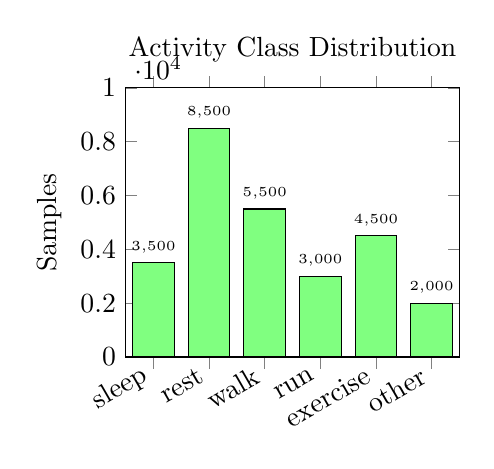
\begin{tikzpicture}
\begin{axis}[
    ybar,
    bar width=15pt,
    ylabel={Samples},
    symbolic x coords={sleep, rest, walk, run, exercise, other},
    xtick=data,
    x tick label style={rotate=30, anchor=east},
    ymin=0, ymax=10000,
    nodes near coords,
    width=0.48\textwidth,
    height=5cm,
    title={Activity Class Distribution},
    every node near coord/.append style={font=\tiny},
]
\addplot[fill=green!50] coordinates {
    (sleep, 3500)
    (rest, 8500)
    (walk, 5500)
    (run, 3000)
    (exercise, 4500)
    (other, 2000)
};
\end{axis}
\end{tikzpicture}
\caption{Activity class distribution in the training dataset.}
\label{fig:activity_dist}
\end{figure}

\subsection{Feature Correlations}

\begin{table}[H]
\centering
\caption{Feature Correlation Matrix}
\label{tab:correlations}
\begin{tabular}{lcccc}
\toprule
& \textbf{HR} & \textbf{Steps} & \textbf{Calories} & \textbf{Distance} \\
\midrule
Heart Rate & 1.000 & 0.683 & 0.742 & 0.651 \\
Steps & 0.683 & 1.000 & 0.891 & 0.934 \\
Calories & 0.742 & 0.891 & 1.000 & 0.876 \\
Distance & 0.651 & 0.934 & 0.876 & 1.000 \\
\bottomrule
\end{tabular}
\end{table}

Steps and distance show the highest correlation (0.934), as expected from the physical relationship.

\section{Validation}

\subsection{Medical Reference Range Compliance}

\begin{table}[H]
\centering
\caption{Synthetic Data vs. Medical Reference Ranges}
\label{tab:medical_validation}
\begin{tabular}{lccc}
\toprule
\textbf{Parameter} & \textbf{Reference} & \textbf{Synthetic ($\mu$)} & \textbf{Match} \\
\midrule
Resting HR & 60--100 BPM & 70.2 BPM & Yes \\
Sleep HR & 40--60 BPM & 55.1 BPM & Yes \\
Exercise HR & 100--170 BPM & 135.4 BPM & Yes \\
Max HR (healthy) & $\leq$ 220-age & $\leq$ 180 BPM & Yes \\
Daily steps & 5K--10K & 6,840 & Yes \\
\bottomrule
\end{tabular}
\end{table}

\subsection{Model Performance on Synthetic Data}

\begin{figure}[H]
\centering
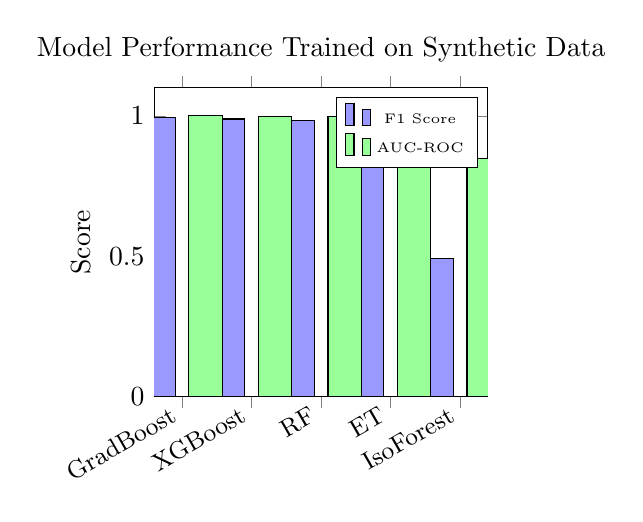
\begin{tikzpicture}
\begin{axis}[
    ybar=5pt,
    bar width=12pt,
    ylabel={Score},
    symbolic x coords={GradBoost, XGBoost, RF, ET, IsoForest},
    xtick=data,
    x tick label style={rotate=30, anchor=east, font=\small},
    ymin=0, ymax=1.1,
    legend pos=north east,
    legend style={font=\tiny},
    width=0.48\textwidth,
    height=5.5cm,
    title={Model Performance Trained on Synthetic Data},
]
\addplot[fill=blue!40] coordinates {
    (GradBoost, 0.995)
    (XGBoost, 0.989)
    (RF, 0.983)
    (ET, 0.966)
    (IsoForest, 0.491)
};
\addlegendentry{F1 Score}
\addplot[fill=green!40] coordinates {
    (GradBoost, 1.000)
    (XGBoost, 0.999)
    (RF, 0.999)
    (ET, 0.999)
    (IsoForest, 0.848)
};
\addlegendentry{AUC-ROC}
\end{axis}
\end{tikzpicture}
\caption{ML model performance achieved with synthetic training data.}
\label{fig:model_perf}
\end{figure}

\subsection{Scenario Test Results}

\begin{table}[H]
\centering
\caption{Scenario-Based Validation Results (Gradient Boosting)}
\label{tab:scenario_results}
\begin{tabular}{lccc}
\toprule
\textbf{Scenario} & \textbf{Samples} & \textbf{Expected} & \textbf{Correct (\%)} \\
\midrule
Normal rest (HR 70-75) & 500 & No alert & 99.8\% \\
Normal exercise (HR 130-145) & 500 & No alert & 99.6\% \\
Tachycardia (HR 150-180 + rest) & 500 & Alert & 99.4\% \\
Bradycardia (HR 30-45 + rest) & 500 & Alert & 99.2\% \\
Exercise spike (HR 150 + exercise) & 500 & No alert & 98.8\% \\
\bottomrule
\end{tabular}
\end{table}

\subsection{Normal vs Anomaly Separation}

\begin{figure}[H]
\centering
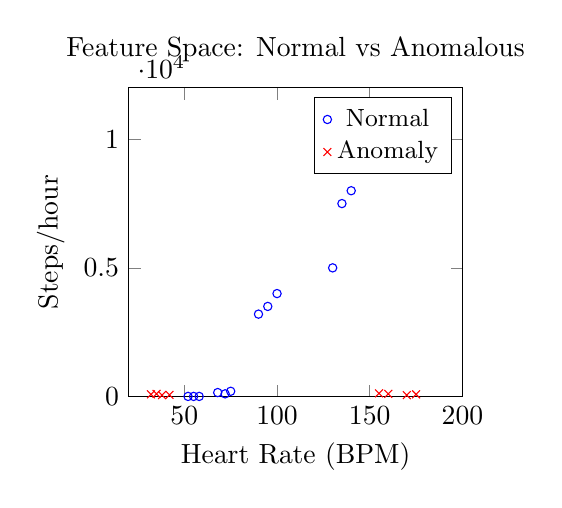
\begin{tikzpicture}
\begin{axis}[
    xlabel={Heart Rate (BPM)},
    ylabel={Steps/hour},
    xmin=20, xmax=200,
    ymin=0, ymax=12000,
    legend pos=north east,
    legend style={font=\small},
    width=0.48\textwidth,
    height=5.5cm,
    title={Feature Space: Normal vs Anomalous},
    scatter/classes={
        normal={mark=o, draw=blue, mark size=1.5pt},
        anomaly={mark=x, draw=red, mark size=2pt}
    },
]
\addplot[scatter, only marks, scatter src=explicit symbolic]
coordinates {
    (72, 100) [normal]
    (68, 150) [normal]
    (75, 200) [normal]
    (95, 3500) [normal]
    (90, 3200) [normal]
    (100, 4000) [normal]
    (140, 8000) [normal]
    (135, 7500) [normal]
    (130, 5000) [normal]
    (55, 0) [normal]
    (58, 0) [normal]
    (52, 0) [normal]
    (160, 100) [anomaly]
    (170, 50) [anomaly]
    (175, 80) [anomaly]
    (155, 120) [anomaly]
    (35, 100) [anomaly]
    (38, 50) [anomaly]
    (32, 80) [anomaly]
    (42, 60) [anomaly]
};
\addlegendentry{Normal}
\addlegendentry{Anomaly}
\end{axis}
\end{tikzpicture}
\caption{2D scatter plot showing separation between normal and anomalous samples in HR-Steps feature space.}
\label{fig:scatter}
\end{figure}

\section{Limitations and Real-World Transition}

\subsection{Current Limitations}
\begin{enumerate}
    \item \textbf{Simplified distributions}: Real vital signs exhibit more complex patterns (diurnal variations, day-to-day variability, medical conditions).
    \item \textbf{Feature independence}: Inter-feature correlations in synthetic data may not perfectly match real sensor data.
    \item \textbf{Missing noise patterns}: Real sensor noise (motion artifacts, skin contact issues) is not modeled.
    \item \textbf{Population diversity}: Current models use a single population profile; real users vary by age, fitness, and health conditions.
\end{enumerate}

\subsection{Transition Strategy}
The transition from synthetic to real data follows a staged approach:
\begin{enumerate}
    \item \textbf{Phase 1 (Current)}: Train on synthetic data, validate on synthetic scenarios.
    \item \textbf{Phase 2}: Collect real data from Wear OS devices (pilot study with 10--20 users).
    \item \textbf{Phase 3}: Fine-tune models on mixed synthetic + real data.
    \item \textbf{Phase 4}: Train primarily on real data, use synthetic for augmentation and edge cases.
\end{enumerate}

\section{Conclusion}
We presented a synthetic health data generation pipeline that produces physiologically realistic training data for wearable health monitoring ML models. The generator creates 27,000 samples across six activity states and four anomaly scenarios, enabling models to achieve F1=0.995 (Gradient Boosting) and 85.8\% accuracy (XGBoost). The context-aware approach ensures that identical vital sign values receive different labels based on activity context (e.g., HR 150 during exercise vs. at rest). Future work includes modeling diurnal vital sign variations, sensor-specific noise patterns, population diversity (age/fitness/health stratification), and transitioning to real-world data collection.

\begin{thebibliography}{00}
\bibitem{synthetic_health} J. Chaopraser and A. Bataineh, ``Synthetic health data generation using generative adversarial networks,'' \textit{BMC Medical Informatics}, vol. 21, p. 188, 2021.
\bibitem{aha_hr} American Heart Association, ``Target heart rates chart,'' \textit{AHA Guidelines}, 2023.
\bibitem{data_aug} T. Iwana and S. Uchida, ``Time series data augmentation for deep learning: A survey,'' \textit{Int. J. of Digital Earth}, vol. 14, no. 8, pp. 1--37, 2021.
\end{thebibliography}

\end{document}
